\documentclass[hyperref=colorlinks]{beamer}
\mode<presentation>
\usetheme{iclpt}
\setbeamertemplate{navigation symbols}{}
\setbeamertemplate{headline}{
  \begin{beamercolorbox}[leftskip=.2cm,rightskip=.2cm,topskip=.2cm,ht=1.1cm,dp=0.1cm,wd=\textwidth]{institute in head/foot}
    
\includegraphics[height=1cm]{icl.pdf}
    \hfill
%    \includegraphics[height=1cm]{../Pics/ATLAS-Logo-Square-Blue-RGB.png}
%    
\includegraphics[height=1cm]{../Pics/CMS-Color.pdf}
    
\includegraphics[height=1cm]{TalkPics/t2k_logo_large.png}

%??put t2k logo here
  \end{beamercolorbox}
}
\setbeamertemplate{footline}{
  \begin{beamercolorbox}[ht=.35cm,dp=0.2cm,wd=\textwidth,leftskip=.3cm]{author in head/foot}%
    \begin{minipage}[c]{5cm}%
      \usebeamerfont{author in head/foot}
      \insertshortauthor 
      \insertshorttitle
    \end{minipage}\hfill%
    \hfill
%    \insertframenumber{} / \ref{lastframe}
    %\hfill
    \begin{minipage}{6cm}
      \hfill
      %\insertshorttitle
    \end{minipage}
  \end{beamercolorbox}%
}

\definecolor{beamer@icdarkblue}{RGB}{0,51,102}
\definecolor{beamer@icmiddleblue}{RGB}{0,82,150} 
\definecolor{beamer@iclightblue}{RGB}{200,212,232}
\definecolor{beamer@icmiddlered}{RGB}{204,51,0}
\definecolor{beamer@iclightred}{RGB}{232,212,32}

\usepackage{tikz}
\usetikzlibrary{arrows,shapes,backgrounds}
\usepackage{color}
\usepackage{tabularx,colortbl}
\usepackage{graphicx}
\usepackage{pdfpages}
\usepackage{feynmp}
\usepackage{rotating}
\usepackage{moresize}
\usepackage{slashed}
\usepackage{xcolor,colortbl}
\DeclareGraphicsRule{*}{mps}{*}{}
\hypersetup{colorlinks=false}

\title[MaCh3 and HPTPC]{\vspace{-0.2cm} MaCh3 and HPTPC}
\author[P. Dunne]{Patrick Dunne - Imperial College London}
\titlegraphic{
  \vspace{-0.4cm}
}
\date{}
\begin{document}
\tikzstyle{every picture}+=[remember picture]
\tikzstyle{na} = [baseline=-.5ex]
\begin{fmffile}{t2ktemplatefeyndiags}


  %TITLE PAGE
  %20 mins + 5 questions
  \section{Title}
  \begin{frame}
    \titlepage
  \end{frame}

  \begin{frame}
    \frametitle{MaCh3 - (Ma)rkov (Ch)ain 3 flavour}
    \begin{columns}
      \column{1.1\textwidth}
      \begin{itemize}
      \item MaCh3 is one of T2K's oscillation fitters
      \item[-] We analyse ND280 and SK data to constrain PMNS parameters
      \item[-] Use Bayesian methods and Markov Chain Monte Carlo
      \item Latest results show exclusion of CP conservation at nearly 90\% confidence and some tension with the PMNS model
      \item Exciting times ahead with lots more data expected
      \end{itemize}
      \end{columns}
    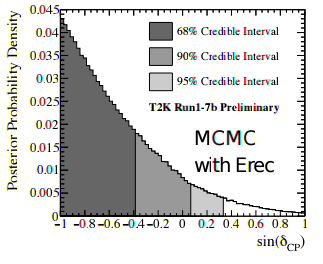
\includegraphics[width=.5\textwidth,height=.4\textheight]{TalkPics/newstudenttalk_pdunne_281116/mach3fit.png}
    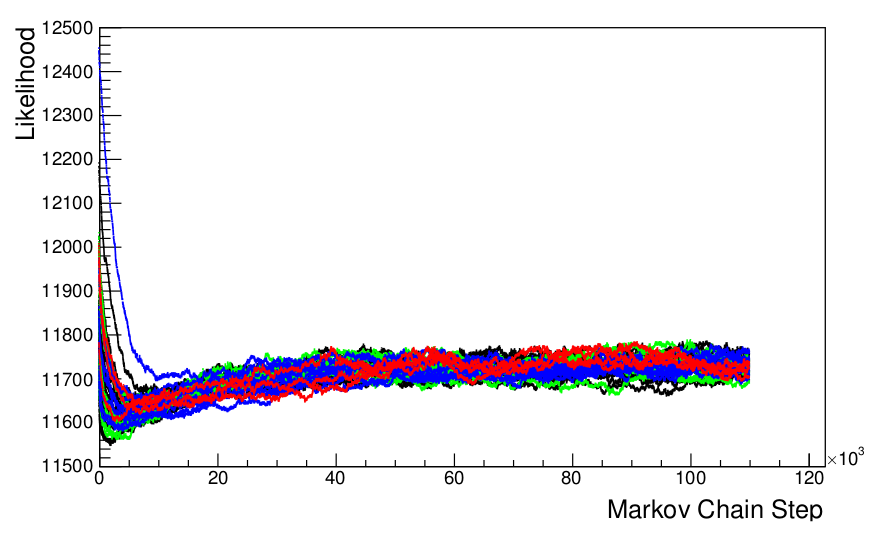
\includegraphics[width=.5\textwidth,height=.4\textheight,clip=true,trim=0 0 0 30 ]{TalkPics/newstudenttalk_pdunne_281116/likelihoodvsstep.pdf}
  \end{frame}

  \begin{frame}
    \label{lastframe}
    \frametitle{High Pressure TPC (HPTPC)}
    \begin{columns}
      \column{1.1\textwidth}
      \begin{itemize}
      \item TPC's allow very good particle ID and low momentum thresholds
      \item[-] Increases hadron information available for analysis
      \item Problem is that gas isn't very dense so interaction rate is low
      \item Using high pressure gas increases density and also interaction rate
      \item HPTPC demonstrator being built in London that will be being tested in beams at CERN
      \end{itemize}
    \end{columns}
      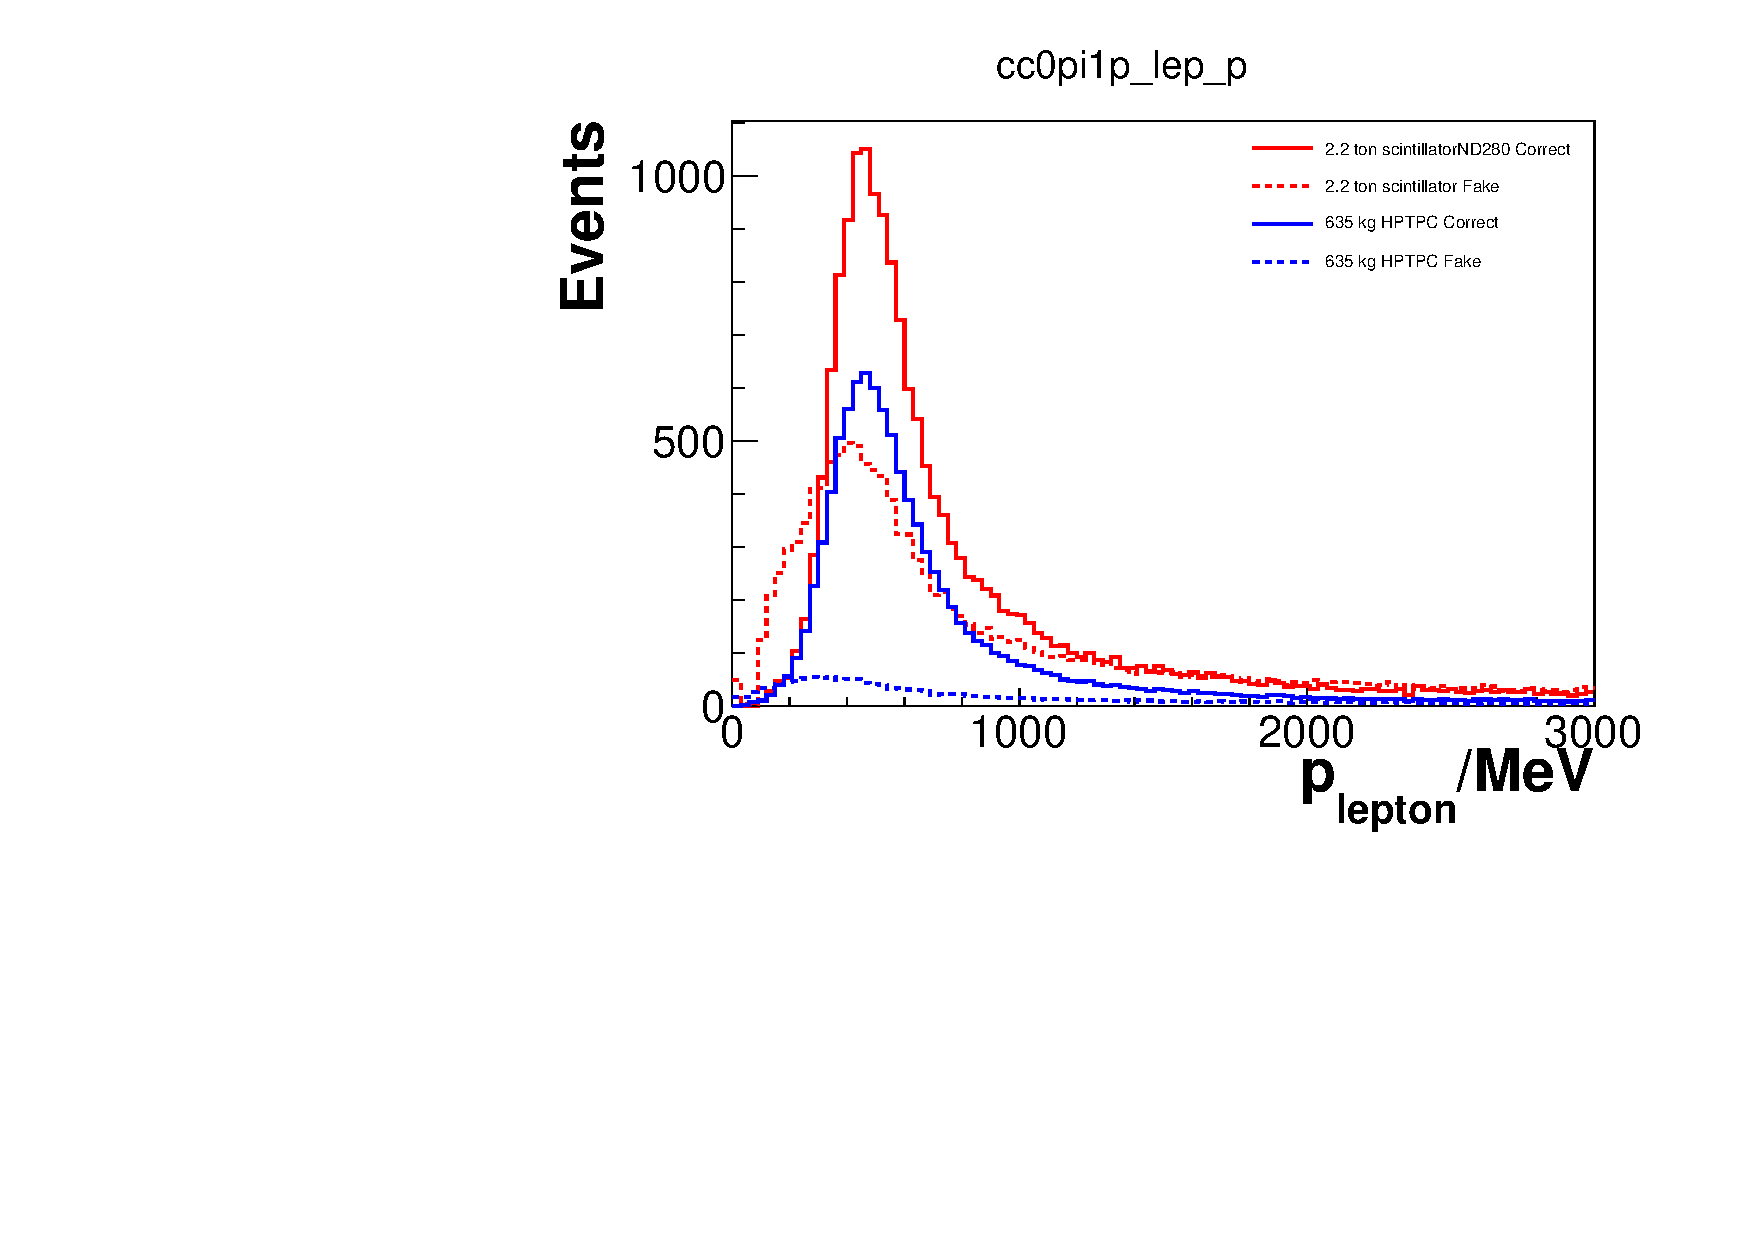
\includegraphics[width=.5\textwidth,height=.4\textheight]{TalkPics/newstudenttalk_pdunne_281116/cc0pi1p_lep_p.pdf}
    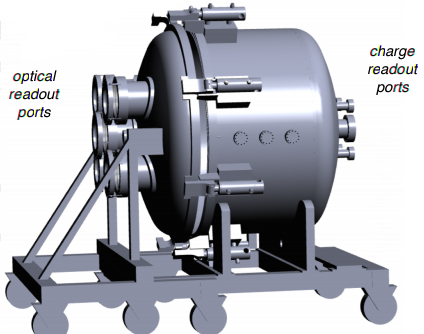
\includegraphics[width=.5\textwidth,height=.4\textheight]{TalkPics/newstudenttalk_pdunne_281116/hptpc.png}
  \end{frame}

  %Backup goes here
  
\end{fmffile}
\end{document}

\begin{frame}
\end{frame}
